Given the above model, our goal is to find the maximum \emph{a posteriori} (MAP) spike train, i.e., the most likely spike train, $\hbn$,  given the fluorescence measurements, $\bF$. Formally, we have:

\begin{align} \label{eq:nhat1} 
\hbn &=  \anx P[\bn | \bF], % =  \anx \frac{1}{P[\bF]} P[\bF | \bn] P[\bn] =  \anx  P[\bF | \bn] P[\bn]   %\\
\end{align}

\noindent where $P[\bn | \bF]$ is the posterior probability of a spike train, $\bn$, given the fluorescent trace, $\bF$, and $n_t$ is constrained to be an integer ($\mathbb{N}_0=\{0,1,2,\ldots\}$).  From Bayes' Rule, we know that we can rewrite the posterior:

\begin{align} \label{eq:bayes}
P[\bn | \bF] = \frac{P[\bn, \bF]}{P[\bF]} = \frac{1}{P[\bF]} P[\bF | \bn] P[\bn],
\end{align}

\noindent where $P[\bF]$ is the evidence of the data; $P[\bF | \bn]$ is the likelihood of a observing a particular fluorescence trace $\bF$, given the spike train $\bn$, and $P[\bn]$ is the prior probability of a spike train.  Plugging Eq. \eqref{eq:bayes} into Eq. \eqref{eq:nhat1}, we have:

\begin{align} \label{eq:nhat2} 
\hbn &=  \anx \frac{1}{P[\bF]} P[\bF | \bn] P[\bn] =  \anx  P[\bF | \bn] P[\bn],
%\\ &=  \anx  P[\bF | \bC] P[\bC] 
\end{align}

\noindent where the second equality follows because $P[\bF]$ merely scales the results, but does not change the relative quality of various spike trains. %, and the third equality follows from the assumed deterministic relationship between $\bn$ and $\bC$ (c.f. Eq. \eqref{eq:C}).  
Fortunately, both $P[\bF | \bn]$ and $P[\bn]$ are available from the above model:

\begin{subequations} \label{eq:post1}
\begin{align}
P[\bF | \bn]&= P[\bF | \bC] 	= \prod_t P[F_t | C_t], \label{eq:lik1} \\ % = 
P[\bn] 		&= \prod_t P[n_t], \label{eq:prior1}% 	= \prod_t 
\end{align}
\end{subequations}

\noindent where the first equality in Eq. \eqref{eq:lik1} follows because $\bC$ is deterministic given $\bn$, and the second equality follows from Eq. \eqref{eq:F}. Further, Eq. \eqref{eq:prior1} follows from the Poisson distribution assumption above, Eq. \eqref{eq:n}.  Fortunately, both $P[F_t | C_t]$ and $P[n_t]$ are given by the model:

\begin{subequations} \label{eq:post2}
\begin{align}
P[F_t | C_t] &= \mN(F_t; \alpha(C_t+\beta),\sig^2), \label{eq:lik2} \\
P[n_t] &= \text{Poisson}(n_t; \lam \Del). \label{eq:prior2} 
\end{align}
\end{subequations}

\noindent where $\mN(x;\mu,\sig^2)$ indicates $x$ has a Gaussian distribution with mean $\mu$ and variance $\sig^2$ and Poisson$(x;k)$ indicates that $x$ has a Poisson distribution with rate $k$, and both equations follow from the above model.  
%\noindent where both Eq. \eqref{eq:lik} and \eqref{eq:prior} follow from the model.  
% 
% A careful analysis of the above model, Eqs. \eqref{eq:F}--\eqref{eq:n}, suggests that we have a \emph{state-space model} \cite{DurbinKoopman01}:
% 
% \begin{subequations} \label{eq:ssm}
% \begin{align} 
% F_t &= \alpha (C_t + \beta) + \sig \varepsilon_t, \qquad& \varepsilon_t \overset{iid}{\sim} \mN(0,1) \\
% C_t &= \gam C_{t-1} + n_t, & n_t \overset{iid}{\sim} \text{Poiss}(\lam \Del)
% \end{align}
% \end{subequations}
% 
% \noindent where $\gam = 1-\tau/\Del$, and $n_t$ has been rescaled appropriately.  We use the above formulation to simplify Eq. \eqref{eq:nhat1}:
% \noindent 
Now, plugging Eq. \eqref{eq:post2} back into \eqref{eq:post1}, and plugging that result into Eq. \eqref{eq:nhat2}, yields:

\begin{subequations}  \label{eq:obj}
\begin{align}
\hbn 	&= \anx \prod_t \frac{1}{\sqrt{2 \pi \sig^2}} \left(-\frac{1}{2}\frac{(F_t - \alpha (C_t + \beta))^2}{\sig^2}\right) \frac{\text{e}^{-\lam\Del} (\lam\Del)^{n_t}}{n_t!}
%&= \argmax_{n_t \in \mathbb{N}_0 \forall t} \prod_{t=1}^T  P[F_t | C_t]  P[C_t | C_{t-1}]  \label{eq:nhat2} \\
%&= \argmax_{n_t \in \mathbb{N}_0 \forall t} \prod_{t=1}^T  P[F_t | C_t]  P[n_t] 
%\label{eq:nhat2}
%= \argmax_{n_t \in \mathbb{N}_0 \forall t} \sum_{t=1}^T \big( \log P[F_t | C_t] + \log P[n_t]\big)  \label{eq:nhat2} %\\
%&= \anx  \sum_{t=1}^T \bigg( \frac{1}{2 \sig^2}(F_t - \alpha(C_t + \beta))^2  -  n_t \log \lam \Del + \log n_t! \bigg), \label{eq:nhat4}   
%\end{align} 
%\end{subequations}
%
%\noindent where Eq. \eqref{eq:nhat1} follows from Eq. \eqref{eq:ssm}, and Eq. \eqref{eq:nhat2} follows from Eq. \eqref{eq:C}. Plugging Eqs. \eqref{eq:F} and \eqref{eq:n} into Eq. \eqref{eq:nhat2} yields:
%
%\begin{align} \label{eq:MAP}
%\bn_{MAP} 
\label{eq:obj1}\\ &= \anx  \sum_t \bigg( -\frac{1}{2 \sig^2}(F_t - \alpha(C_t + \beta))^2  -  n_t \log \lam \Del + \log n_t! \bigg), \label{eq:logobj1}
\end{align} 
\end{subequations}

\noindent where the second equality follows from taking the logarithm of the right-hand-side.  Unfortunately, solving Eq. \eqref{eq:logobj1} exactly is computationally intractable, as it requires a nonlinear search over an infinite number of  possible spike trains.  We could restrict our search space by imposing an upper bound, $k$, on the number of spikes within a frame.  However, in that case, the computational complexity scales \emph{exponentially} with the number of image frames --- i.e., the number of computations required would scale with $k^T$ --- which for pragmatic reasons is intractable.  Thus, we approximate Eq. \eqref{eq:obj}, by modifying Eq. \eqref{eq:n}, replacing the Poisson distribution with an exponential distribution.  The advantage of this approximation is that the optimization problem becomes log-concave, meaning that we can use any gradient ascent method to guarantee that we achieve the global maximum (because there are no local maxima, other than the single global maximum).  The disadvantage, however, is that we lose the constraint of integer results, i.e., we allow for our answer to include ``partial'' spikes.  This ``disadvantage'' can be remedied by thresholding, or by considering the magnitude of a partial spike as the probability of a spike occurring in that time bin.  We discuss this in more detail in the Discussion section. 

%
%This reduces the algorithmic complexity from requiring a search over $\approx k^T$ possible spike trains, to polynomial complexity, i.e., $\approx T^p$, where $p$ depends on the precise details of the algorithm.  
%
%Two distributions naturally arise as possible approximations to a Poisson: (i) exponential, and (ii) Gaussian.  As depicted in Figure \ref{fig:dist_comp}  an exponential distribution (dashed gray line) is an excellent approximation to the Poisson distribution (solid black line), when $\lam$ is small (left panel).  On the other hand, when $\lam$ is large, a Gaussian distribution (dash-dotted gray line) closely approximates a Poisson when $\lam$ is large (right panel). Thus, \nai vely, it seems as though it may be desirable to use a Gaussian approximation when the neuron is firing with a high firing rate, and approximate the Poisson with an exponential when the neuron is firing sparsely.  The Wiener filter is, in fact, the optimal filter given the Gaussian approximation \cite{Wiener49} (see \cite{HolekampHoly08} for an application of the Wiener filter to this problem).  Below, we develop an algorithm to perform inference given the exponential distribution.  
%
% \begin{figure}[h!]
% \centering 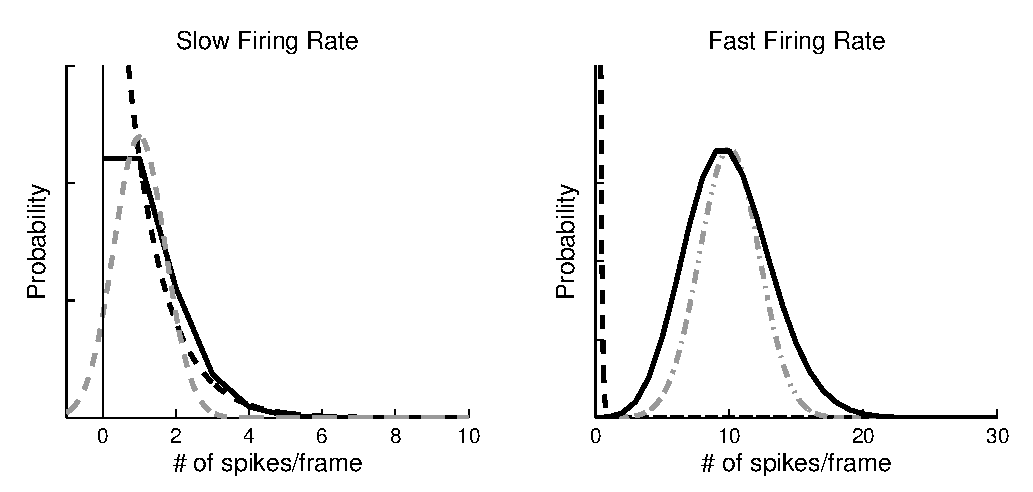
\includegraphics[width=.9\linewidth]{../figs/dist_comp}
% \caption{Approximating a Poisson distribution.  Left panel: when $\lam$ is small (e.g., $\approx 1$), an exponential distribution (dashed gray line) approximates the Poisson distribution (solid black line) well, but a Gaussian distribution (dash-dotted gray line) does not.  Right panel: when $\lam$ is large (e.g., $\approx 20$), the inverse is true.} \label{fig:dist_comp}
% \end{figure}